\documentclass[12pt,a4paper]{article}
\usepackage[a4paper, top=0.8in, bottom=1.1in, left=0.8in, right=0.8in, headheight=14pt, footskip=30pt]{geometry}
\usepackage{fontspec}
\usepackage{unicode-math}
\setmainfont{TeX Gyre Pagella}
\setmonofont[Scale=0.88]{TeX Gyre Cursor}
\setmathfont{Latin Modern Math}
\usepackage{xcolor}
\usepackage{titlesec}
\usepackage{enumitem}
\usepackage{tabularx}
\usepackage{booktabs}
\usepackage{array}
\usepackage{amsmath}
\usepackage{tikz}
\usetikzlibrary{shapes.geometric, arrows.meta, positioning, calc, fit, decorations.pathreplacing, decorations.pathmorphing}
\usepackage{tcolorbox}
\tcbuselibrary{skins, breakable}
\usepackage{hyperref}
\usepackage{fancyhdr}
\usepackage{graphicx}
\usepackage{microtype}
\hyphenpenalty=10000
\exhyphenpenalty=10000
\sloppy
\usepackage{caption}
\usepackage{setspace}
\usepackage{multirow}
\usepackage{tocloft}
\newcommand{\Q}[1]{\textbf{#1}\par\noindent\ignorespaces}
\definecolor{myred}{RGB}{196,30,58}
\definecolor{mydark}{RGB}{30,30,50}
\definecolor{mygreen}{RGB}{14,120,80}
\definecolor{myteal}{RGB}{0,130,140}
\definecolor{myamber}{RGB}{180,100,0}
\definecolor{mypurple}{RGB}{100,30,160}
\definecolor{mygray}{RGB}{246,247,249}
\definecolor{mgframe}{RGB}{180,185,200}
\definecolor{watermark}{RGB}{145,150,170}
\definecolor{hdrred}{RGB}{250,232,235}
\definecolor{hdrgreen}{RGB}{220,244,233}
\definecolor{hdrteal}{RGB}{220,242,244}
\definecolor{hdramber}{RGB}{253,242,215}
\definecolor{hdrpurple}{RGB}{238,228,255}
\definecolor{hdrgray}{RGB}{238,240,245}
\definecolor{rowalt}{RGB}{250,251,253}
\titleformat{\section}{\large\bfseries\color{myred}}{\thesection.}{0.5em}{}[\vspace{1pt}{\color{myred}\rule{\linewidth}{0.8pt}}]
\titleformat{\subsection}{\normalsize\bfseries\color{myteal}}{\thesubsection}{0.5em}{}
\titlespacing*{\section}{0pt}{18pt}{7pt}
\titlespacing*{\subsection}{0pt}{11pt}{4pt}
\setlength{\parindent}{0pt}
\setlength{\parskip}{4pt}
\raggedbottom
\renewcommand{\cfttoctitlefont}{\large\bfseries\color{myred}}
\renewcommand{\cftaftertoctitle}{\par\noindent{\color{myred}\rule{\linewidth}{0.8pt}}}
\setlength{\cftbeforetoctitleskip}{0pt}
\setlength{\cftaftertoctitleskip}{6pt}
\renewcommand{\cftsecfont}{\normalsize\bfseries\color{mydark}}
\renewcommand{\cftsecpagefont}{\normalsize\bfseries\color{mydark}}
\renewcommand{\cftsecleader}{\cftdotfill{\cftdotsep}}
\setlength{\cftbeforesecskip}{7pt}
\renewcommand{\cftsubsecfont}{\small\color{mydark}}
\renewcommand{\cftsubsecpagefont}{\small\color{mydark}}
\setlength{\cftbeforesubsecskip}{3pt}
\setlength{\cftsubsecindent}{1.4em}
\renewcommand{\arraystretch}{1.45}
\setlength{\tabcolsep}{6pt}
\newcolumntype{B}[1]{>{\small\bfseries\raggedright\arraybackslash}m{#1}}
\newcolumntype{Y}{>{\small\raggedright\arraybackslash}X}
\renewcommand{\tabularxcolumn}[1]{m{#1}}
\pagestyle{fancy}
\fancyhf{}
\fancyhead[L]{\small\color{myred}\textbf{BS-CH101}\;\color{mydark}--- Chemistry-I}
\fancyhead[R]{\small\color{myteal}\textbf{Module 4 Long Notes}}
\fancyfoot[L]{\small\color{watermark}\textit{\copyright\ MAKAUT Wingman}}
\fancyfoot[C]{\small\color{mydark}\thepage}
\fancyfoot[R]{\small\color{watermark}\textit{\copyright\ Biraj}}
\renewcommand{\headrulewidth}{0.5pt}
\renewcommand{\footrulewidth}{0.3pt}
\hypersetup{colorlinks=true, linkcolor=myteal, urlcolor=myteal, pdfauthor={Biraj Sarkar},
  pdftitle={BS-CH101 --- Module 4 Long Notes: Free Energy and Chemical Equilibria}}
\tcbset{
  tikzbox/.style={colback=mygray, colframe=mgframe, boxrule=0.6pt, arc=4pt,
    left=8pt, right=8pt, top=6pt, bottom=6pt, colbacktitle=mgframe, coltitle=mydark, fonttitle=\small\bfseries},
  defbox/.style={colback=hdrgreen, colframe=mygreen, boxrule=0.8pt, arc=4pt,
    left=9pt, right=9pt, top=6pt, bottom=6pt, colbacktitle=mygreen, coltitle=white, fonttitle=\small\bfseries},
  formulabox/.style={colback=hdrteal, colframe=myteal, boxrule=0.8pt, arc=4pt,
    left=9pt, right=9pt, top=7pt, bottom=7pt, colbacktitle=myteal, coltitle=white, fonttitle=\small\bfseries},
  examplebox/.style={colback=hdramber, colframe=myamber, boxrule=0.8pt, arc=4pt,
    left=9pt, right=9pt, top=6pt, bottom=6pt, colbacktitle=myamber, coltitle=white, fonttitle=\small\bfseries},
  masonbox/.style={colback=hdrpurple, colframe=mypurple, boxrule=0.8pt, arc=4pt,
    left=9pt, right=9pt, top=6pt, bottom=6pt, colbacktitle=mypurple, coltitle=white, fonttitle=\small\bfseries},
  exambox/.style={colback=hdrpurple, colframe=mypurple, boxrule=1pt, arc=5pt,
    left=10pt, right=10pt, top=8pt, bottom=8pt, colbacktitle=mypurple, coltitle=white,
    fonttitle=\bfseries, breakable, title after break={\textbf{Frequently Asked / Viva Questions (contd.)}}}
}
\tcbset{breakable}
\tikzset{
  block/.style={rectangle, draw=myteal, fill=hdrteal, text width=2.4cm, align=center,
    minimum height=0.95cm, font=\small, rounded corners=3pt, line width=0.7pt},
  redblock/.style={rectangle, draw=myred, fill=hdrred, text width=2.4cm, align=center,
    minimum height=0.95cm, font=\small, rounded corners=3pt, line width=0.7pt},
  netnode/.style={rectangle, draw=myteal, fill=hdrteal, text width=1.5cm, align=center,
    minimum height=0.8cm, font=\small, rounded corners=3pt, line width=0.7pt},
  sumjunc/.style={circle, draw=myamber, fill=hdramber, minimum size=0.62cm, font=\small, line width=0.8pt},
  snode/.style={circle, draw=mypurple, fill=hdrpurple, minimum size=0.55cm, font=\footnotesize, line width=0.7pt},
  arrow/.style={-Stealth, thick, color=mydark},
  redarrow/.style={-Stealth, thick, color=myred},
  line/.style={thick, color=mydark}
}

\begin{document}
\begin{center}
  {\LARGE\bfseries\color{myred} BS-CH101 / BS-CH201 --- Chemistry-I}\\[5pt]
  {\normalsize\color{mydark} Semester I/II \quad$\bullet$\quad 3L:1T:0P \quad$\bullet$\quad 4 Credits}\\[3pt]
  {\normalsize\color{myteal}\textbf{Module 4 Long Notes: Free Energy and Chemical Equilibria}}\\[3pt]
  {\small\color{mydark} CGEC \;$|$\; B.Tech ECE (2023--27) \;$|$\; \textit{Biraj Sarkar}}
\end{center}
\vspace{2pt}
\noindent{\color{myred}\rule{\linewidth}{1.5pt}}
\vspace{2pt}
\hypersetup{linkcolor=mydark}
\tableofcontents
\hypersetup{linkcolor=myteal}
\newpage
% ===============================================================================
\section{First and Second Laws of Thermodynamics}
% ===============================================================================

\begin{tcolorbox}[defbox]
\textbf{Thermodynamics} is the study of energy transformations. The \emph{first law} states that energy is conserved; the \emph{second law} states that any spontaneous process increases the total entropy of the universe. Together they define the direction and limits of all chemical and physical processes.
\end{tcolorbox}

\subsection{System, Surroundings, and Universe}
\begin{tabularx}{\linewidth}{|B{2.4cm}|Y|Y|}
\hline
\textbf{Term} & \textbf{Definition} & \textbf{Types} \\
\hline
System & The part under study & Open (matter + energy exchange), closed (energy only), isolated (neither) \\
\hline
Surroundings & Everything outside the system & Provides or absorbs heat and work \\
\hline
Universe & System + surroundings & Total energy and entropy defined for universe \\
\hline
\end{tabularx}

\subsection{Internal Energy and the First Law}
\begin{tcolorbox}[formulabox, title={First Law of Thermodynamics}]
\[
\Delta U = q + w
\]
$\Delta U$ = change in internal energy; $q$ = heat absorbed by system (positive when absorbed); $w$ = work done on system.\\
For expansion against constant pressure: $w = -P_{\mathrm{ext}}\,\Delta V$.\\
At constant volume: $\Delta U = q_v$.\\
At constant pressure: $q_p = \Delta H = \Delta U + P\Delta V = \Delta U + \Delta n_g RT$ (for ideal gases).
\end{tcolorbox}

\subsection{Enthalpy and Heat Capacity}
\begin{tcolorbox}[formulabox, title={Enthalpy and Heat Capacity Relations}]
\[
H = U + PV \quad\Rightarrow\quad \Delta H = \Delta U + \Delta(PV)
\]
\[
C_P = \left(\frac{\partial H}{\partial T}\right)_P, \qquad C_V = \left(\frac{\partial U}{\partial T}\right)_V, \qquad C_P - C_V = R\ \text{(ideal gas)}
\]
For a process at constant $P$: $q_P = n C_P \Delta T$.\\
For a process at constant $V$: $q_V = n C_V \Delta T$.
\end{tcolorbox}

\subsection{Hess's Law and Standard Enthalpies}
\begin{tcolorbox}[defbox]
\textbf{Hess's law:} The enthalpy change of a reaction is independent of the pathway; only the initial and final states matter. Thermochemical equations can be combined algebraically to find $\Delta H$ of reactions that are difficult to measure directly.
\end{tcolorbox}

\begin{tcolorbox}[tikzbox, title={Hess's Law Energy Cycle for Combustion of Carbon}]
\centering
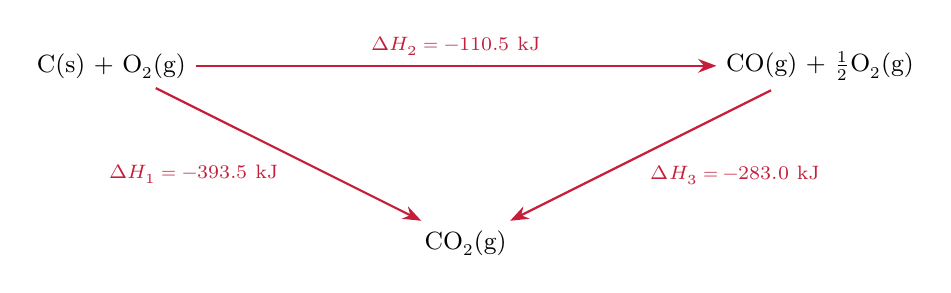
\begin{tikzpicture}[scale=0.9]
  % top-left: C(s) + O2
  \node[font=\small, align=center] (A) at (0,2.5) {C(s) + O$_2$(g)};
  % bottom: CO2(g)
  \node[font=\small, align=center] (B) at (5,0) {CO$_2$(g)};
  % top-right: CO(g) + 1/2 O2
  \node[font=\small, align=center] (C) at (10,2.5) {CO(g) + $\tfrac{1}{2}$O$_2$(g)};
  \draw[redarrow, thick] (A) -- node[below left, font=\scriptsize, color=myred] {$\Delta H_1=-393.5\ \mathrm{kJ}$} (B);
  \draw[redarrow, thick] (A) -- node[above, font=\scriptsize, color=myred] {$\Delta H_2=-110.5\ \mathrm{kJ}$} (C);
  \draw[redarrow, thick] (C) -- node[below right, font=\scriptsize, color=myred] {$\Delta H_3=-283.0\ \mathrm{kJ}$} (B);
\end{tikzpicture}
\end{tcolorbox}

\begin{tcolorbox}[examplebox, title={Solved Example: Hess's Law}]
\textbf{Problem:} Find $\Delta H$ for C(s) + $\tfrac{1}{2}$O$_2$(g) $\to$ CO(g) using:
\begin{enumerate}[leftmargin=*, itemsep=1pt, topsep=1pt]
  \item C(s) + O$_2$(g) $\to$ CO$_2$(g), $\Delta H_1 = -393.5\ \mathrm{kJ\,mol^{-1}}$
  \item CO(g) + $\tfrac{1}{2}$O$_2$(g) $\to$ CO$_2$(g), $\Delta H_2 = -283.0\ \mathrm{kJ\,mol^{-1}}$
\end{enumerate}
\textbf{Solution:} Reverse equation 2 and add:
\[
\Delta H = \Delta H_1 - \Delta H_2 = -393.5 - (-283.0) = -110.5\ \mathrm{kJ\,mol^{-1}}
\]
\end{tcolorbox}

\subsection{Entropy: The Second Law}
\begin{tcolorbox}[defbox]
\textbf{Entropy} $S$ is a state function that measures the dispersal of energy among available microstates. The \textbf{second law} states that for any spontaneous process, $\Delta S_{\mathrm{universe}} = \Delta S_{\mathrm{sys}} + \Delta S_{\mathrm{surr}} > 0$. For a reversible process, $\Delta S_{\mathrm{universe}} = 0$.
\end{tcolorbox}

\begin{tcolorbox}[formulabox, title={Entropy Expressions}]
\[
dS = \frac{\delta q_{\mathrm{rev}}}{T}, \qquad \Delta S = \int_1^2 \frac{\delta q_{\mathrm{rev}}}{T}
\]
For a reversible isothermal expansion of ideal gas: $\Delta S = nR\ln\frac{V_2}{V_1}$.\\
For heating at constant $P$: $\Delta S = nC_P\ln\frac{T_2}{T_1}$.\\
For heating at constant $V$: $\Delta S = nC_V\ln\frac{T_2}{T_1}$.\\
Clausius inequality: $\oint \frac{\delta q}{T} \leq 0$ (equality for reversible cycle).
\end{tcolorbox}

\subsection{Third Law and Absolute Entropy}
\begin{tcolorbox}[defbox]
\textbf{Third law of thermodynamics:} The entropy of a perfect crystalline substance is zero at absolute zero ($S = 0$ at $T = 0\ \mathrm{K}$). This provides an absolute reference scale for entropy.
\end{tcolorbox}

\textbf{Standard molar entropy} $S^\circ$ at 298 K (J mol$^{-1}$ K$^{-1}$):
\begin{tabularx}{\linewidth}{|B{2.6cm}|Y|B{2.6cm}|Y|}
\hline
\textbf{Substance} & \textbf{$S^\circ$} & \textbf{Substance} & \textbf{$S^\circ$} \\
\hline
C(graphite) & 5.7 & H$_2$O(l) & 69.9 \\
\hline
H$_2$(g) & 130.7 & CO$_2$(g) & 213.8 \\
\hline
O$_2$(g) & 205.2 & NaCl(s) & 72.1 \\
\hline
\end{tabularx}

Standard entropy change of reaction: $\Delta S^\circ_{\mathrm{rxn}} = \sum n_p S^\circ(\text{products}) - \sum n_r S^\circ(\text{reactants})$.

\subsection{Work in Reversible and Irreversible Expansion}
This is a 5-mark derivation in nearly every MAKAUT paper.

\begin{tcolorbox}[formulabox, title={Work Done by an Ideal Gas}]
\textbf{Reversible isothermal expansion} (maximum work):
\[
w_{\mathrm{rev}} = -nRT\ln\frac{V_2}{V_1} = -nRT\ln\frac{P_1}{P_2}
\]
\textbf{Irreversible expansion against constant external pressure}:
\[
w_{\mathrm{irrev}} = -P_{\mathrm{ext}}\Delta V = -P_{\mathrm{ext}}(V_2-V_1)
\]
\textbf{Free expansion} (into vacuum, $P_{\mathrm{ext}}=0$): $w = 0$.\\
Rule: $|w_{\mathrm{rev}}| > |w_{\mathrm{irrev}}|$ always — reversible processes deliver maximum work.
\end{tcolorbox}

\begin{tcolorbox}[examplebox, title={Solved Example: Reversible vs Irreversible Work}]
1 mol ideal gas at 300 K expands from $V_1=10\ \mathrm{L}$ to $V_2=30\ \mathrm{L}$.

\textbf{Reversible:}
\[
w_{\mathrm{rev}} = -nRT\ln\frac{V_2}{V_1} = -(1)(8.314)(300)\ln 3 = -2494\times1.099 = -2741\ \mathrm{J}
\]
\textbf{Irreversible} against $P_{\mathrm{ext}} = P_2 = nRT/V_2 = (1)(8.314)(300)/30\times10^{-3} = 83140\ \mathrm{Pa}$:

$w_{\mathrm{irrev}} = -(83140)(30-10)\times10^{-3} = -1663\ \mathrm{J}$

Reversible work ($2741\ \mathrm{J}$) is greater than irreversible work ($1663\ \mathrm{J}$) — confirms second law.
\end{tcolorbox}

\subsection{Entropy of Phase Transition and Trouton's Rule}
At a phase transition (melting, boiling), temperature is constant and heat flows reversibly:
\[
\Delta S_{\mathrm{vap}} = \frac{\Delta H_{\mathrm{vap}}}{T_b}, \qquad \Delta S_{\mathrm{fus}} = \frac{\Delta H_{\mathrm{fus}}}{T_m}
\]
\textbf{Trouton's rule:} For most non-associated liquids, $\Delta S_{\mathrm{vap}} \approx 85\ \mathrm{J\,mol^{-1}\,K^{-1}}$ at the normal boiling point. Water deviates ($\Delta S_{\mathrm{vap}} \approx 109\ \mathrm{J\,mol^{-1}\,K^{-1}}$) because its extensive H-bonding creates extra order in the liquid phase.

\subsection{Kirchhoff's Equation: ΔH Variation with Temperature}
Enthalpy of a reaction changes with temperature because reactant and product heat capacities differ.

\begin{tcolorbox}[formulabox, title={Kirchhoff's Equation}]
\[
\frac{d(\Delta H)}{dT} = \Delta C_P = \sum n_p C_P(\text{products}) - \sum n_r C_P(\text{reactants})
\]
Integrated form (assuming $\Delta C_P$ is constant):
\[
\Delta H_{T_2} = \Delta H_{T_1} + \Delta C_P\,(T_2 - T_1)
\]
\end{tcolorbox}

\begin{tcolorbox}[exambox, title={Exam Points (Section 1)}]
\begin{itemize}[leftmargin=*, itemsep=2pt, topsep=2pt]
  \item First law: $\Delta U = q + w$; at const $P$: $\Delta H = q_P$.
  \item $C_P - C_V = R$ for ideal gas; $\Delta H = \Delta U + \Delta n_g RT$ for gas reactions.
  \item Hess's law: $\Delta H$ is path-independent; combine equations algebraically.
  \item Second law: $\Delta S_{\mathrm{univ}} > 0$ for spontaneous; $= 0$ reversible.
  \item Third law: $S = 0$ at $0\ \mathrm{K}$ for perfect crystal — provides absolute entropy scale.
\end{itemize}
\end{tcolorbox}

% ===============================================================================
\section{Gibbs Free Energy and Spontaneity}
% ===============================================================================

\begin{tcolorbox}[defbox]
\textbf{Gibbs free energy} $G = H - TS$ is the thermodynamic potential that determines spontaneity at constant temperature and pressure. It combines both the enthalpic driving force (energy minimisation) and the entropic driving force (disorder maximisation) into a single criterion.
\end{tcolorbox}

\subsection{Derivation of the Gibbs Free Energy Criterion}
At constant $T$ and $P$, the second law requires $\Delta S_{\mathrm{univ}} \geq 0$. Since $\Delta S_{\mathrm{surr}} = -\Delta H / T$ (heat lost by system is gained by surroundings reversibly):
\[
\Delta S_{\mathrm{univ}} = \Delta S_{\mathrm{sys}} - \frac{\Delta H}{T} \geq 0
\quad\Rightarrow\quad T\Delta S - \Delta H \geq 0
\quad\Rightarrow\quad \Delta H - T\Delta S \leq 0
\]
Defining $\Delta G = \Delta H - T\Delta S$:

\begin{tcolorbox}[formulabox, title={Gibbs Free Energy Criterion}]
\[
\Delta G = \Delta H - T\Delta S
\]
\begin{itemize}[leftmargin=*, itemsep=1pt, topsep=2pt]
  \item $\Delta G < 0$: spontaneous (product-favoured).
  \item $\Delta G = 0$: system at equilibrium.
  \item $\Delta G > 0$: non-spontaneous (reactant-favoured under those conditions).
\end{itemize}
$\Delta G$ equals the maximum non-expansion (useful) work: $w_{\mathrm{max}} = \Delta G$.
\end{tcolorbox}

\subsection{The Four Spontaneity Cases}
The sign of $\Delta G = \Delta H - T\Delta S$ depends on temperature through the entropy term.

\begin{tabularx}{\linewidth}{|B{1.8cm}|B{1.8cm}|Y|Y|}
\hline
\textbf{$\Delta H$} & \textbf{$\Delta S$} & \textbf{Sign of $\Delta G$} & \textbf{Spontaneity} \\
\hline
$-$ & $+$ & Always $-$ & Spontaneous at \textbf{all} temperatures \\
\hline
$+$ & $-$ & Always $+$ & Non-spontaneous at \textbf{all} temperatures \\
\hline
$-$ & $-$ & $-$ at low $T$, $+$ at high $T$ & Spontaneous at \textbf{low} temperature \\
\hline
$+$ & $+$ & $+$ at low $T$, $-$ at high $T$ & Spontaneous at \textbf{high} temperature \\
\hline
\end{tabularx}

\textbf{Crossover temperature} (where $\Delta G = 0$):
\[
T^* = \frac{\Delta H}{\Delta S}
\]

\begin{tcolorbox}[examplebox, title={Solved Example: Crossover Temperature}]
For the decomposition of $\mathrm{CaCO_3}(s) \to \mathrm{CaO}(s) + \mathrm{CO_2}(g)$:
$\Delta H^\circ = +178\ \mathrm{kJ\,mol^{-1}}$, $\Delta S^\circ = +165\ \mathrm{J\,mol^{-1}\,K^{-1}} = +0.165\ \mathrm{kJ\,mol^{-1}\,K^{-1}}$.
\[
T^* = \frac{178}{0.165} = 1079\ \mathrm{K}
\]
Below 1079 K the reaction is non-spontaneous ($\Delta G > 0$); above it becomes spontaneous ($\Delta G < 0$). This explains why limestone kilns operate above $\sim 800^\circ\mathrm{C}$.
\end{tcolorbox}

\subsection{Standard Free Energy of Formation}
\begin{tcolorbox}[defbox]
$\Delta G_f^\circ$ is the Gibbs free energy change when one mole of a compound is formed from its elements in their standard states at 298 K and 1 bar. By definition, $\Delta G_f^\circ = 0$ for all elements in their standard states.
\end{tcolorbox}

\[
\Delta G^\circ_{\mathrm{rxn}} = \sum n_p\,\Delta G_f^\circ(\text{products}) - \sum n_r\,\Delta G_f^\circ(\text{reactants})
\]

\begin{tabularx}{\linewidth}{|B{3.2cm}|Y|B{3.2cm}|Y|}
\hline
\textbf{Substance} & \textbf{$\Delta G_f^\circ$ (kJ/mol)} & \textbf{Substance} & \textbf{$\Delta G_f^\circ$ (kJ/mol)} \\
\hline
H$_2$O(l) & $-237.1$ & CO$_2$(g) & $-394.4$ \\
\hline
CO(g) & $-137.2$ & NH$_3$(g) & $-16.5$ \\
\hline
HCl(g) & $-95.3$ & NO(g) & $+86.6$ \\
\hline
\end{tabularx}

\subsection{Temperature Dependence: Gibbs--Helmholtz Equation}
How does $\Delta G$ change with temperature?

\begin{tcolorbox}[formulabox, title={Gibbs--Helmholtz Equation}]
\[
\left(\frac{\partial(\Delta G/T)}{\partial T}\right)_P = -\frac{\Delta H}{T^2}
\]
Integrated form (assuming $\Delta H$ is independent of $T$):
\[
\frac{\Delta G_2}{T_2} - \frac{\Delta G_1}{T_1} = -\Delta H\!\left(\frac{1}{T_2} - \frac{1}{T_1}\right)
\]
Used to calculate $\Delta G$ at a new temperature $T_2$ from a known value at $T_1$.
\end{tcolorbox}

\begin{tcolorbox}[examplebox, title={Solved Example: \texorpdfstring{$\Delta G$}{Delta G} at New Temperature}]
$\Delta G^\circ_{298} = -33.0\ \mathrm{kJ\,mol^{-1}}$, $\Delta H^\circ = -92.0\ \mathrm{kJ\,mol^{-1}}$ for $\mathrm{N_2 + 3H_2 \to 2NH_3}$.
Find $\Delta G^\circ$ at 500 K:
\[
\frac{\Delta G^\circ_{500}}{500} - \frac{-33000}{298} = -(-92000)\!\left(\frac{1}{500} - \frac{1}{298}\right)
\]
\[
\frac{\Delta G^\circ_{500}}{500} + 110.7 = 92000\times\frac{202}{149000} = 124.8
\]
\[
\Delta G^\circ_{500} = (124.8 - 110.7)\times 500 = +7050\ \mathrm{J\,mol^{-1}} = +7.1\ \mathrm{kJ\,mol^{-1}}
\]
The reaction becomes non-spontaneous above $\sim 460\ \mathrm{K}$ (industrial Haber process must use a catalyst to achieve acceptable rate below this temperature).
\end{tcolorbox}

\begin{tcolorbox}[exambox, title={Exam Points (Section 2)}]
\begin{itemize}[leftmargin=*, itemsep=2pt, topsep=2pt]
  \item Derive $\Delta G = \Delta H - T\Delta S$ from the second law at constant $T$, $P$.
  \item Quote all 4 sign-of-$\Delta G$ cases; always give the temperature condition.
  \item Crossover temperature: $T^* = \Delta H/\Delta S$ (units: J cancel, gives K directly if both in J).
  \item $\Delta G^\circ_{\mathrm{rxn}}$ from formation free energies: products minus reactants.
  \item Gibbs--Helmholtz: $(\partial(\Delta G/T)/\partial T)_P = -\Delta H/T^2$.
\end{itemize}
\end{tcolorbox}

% ===============================================================================
\section{Free Energy and Chemical Equilibrium}
% ===============================================================================

\begin{tcolorbox}[defbox]
At equilibrium, the Gibbs free energy of a reacting mixture reaches its minimum value. The standard free energy change $\Delta G^\circ$ is directly related to the equilibrium constant $K$ through $\Delta G^\circ = -RT\ln K$, providing the fundamental link between thermodynamics and equilibrium chemistry.
\end{tcolorbox}

\subsection{Chemical Potential and Reaction Quotient}
For an ideal gas species $i$ at partial pressure $P_i$, the chemical potential is:
\[
\mu_i = \mu_i^\circ + RT\ln\frac{P_i}{P^\circ}
\]
For a reaction $a\mathrm{A} + b\mathrm{B} \to c\mathrm{C} + d\mathrm{D}$, the free energy change is:
\[
\Delta G = \Delta G^\circ + RT\ln Q
\]
where the reaction quotient $Q = \frac{[C]^c[D]^d}{[A]^a[B]^b}$ uses current concentrations (or partial pressures).

\subsection{Relationships Between \texorpdfstring{$K_p$, $K_c$, $K_x$}{Kp, Kc, Kx}}
Three forms of the equilibrium constant are commonly used. They are interrelated through the ideal gas law.

\begin{tcolorbox}[formulabox, title={Equilibrium Constant Relationships}]
\[
K_p = K_c\,(RT)^{\Delta n_g}, \qquad K_p = K_x\,P^{\Delta n_g}
\]
$K_p$ = equilibrium constant in terms of partial pressures (bar or atm).\\
$K_c$ = equilibrium constant in terms of molar concentrations (mol L$^{-1}$).\\
$K_x$ = equilibrium constant in terms of mole fractions (dimensionless).\\
$\Delta n_g$ = moles of gaseous products $-$ moles of gaseous reactants.\\
When $\Delta n_g = 0$: $K_p = K_c = K_x$ (e.g.\ $\mathrm{H_2 + I_2 \rightleftharpoons 2HI}$).
\end{tcolorbox}

\begin{tcolorbox}[examplebox, title={Solved Example: \texorpdfstring{$K_p$}{Kp} from \texorpdfstring{$K_c$}{Kc}}]
For $\mathrm{N_2(g) + 3H_2(g) \rightleftharpoons 2NH_3(g)}$ at 500 K, $K_c = 6.0\times10^{-2}\ \mathrm{L^2\,mol^{-2}}$.\\
$\Delta n_g = 2 - (1+3) = -2$.
\[
K_p = K_c\,(RT)^{\Delta n_g} = 6.0\times10^{-2}\times(0.0821\times500)^{-2}
= 6.0\times10^{-2}\times(41.05)^{-2} = 3.55\times10^{-5}\ \mathrm{atm^{-2}}
\]
$K_p < K_c$ because $\Delta n_g < 0$ (fewer moles of gas at equilibrium).
\end{tcolorbox}

\subsection{Derivation of \texorpdfstring{$\Delta G^\circ = -RT\ln K$}{Delta G0 = -RT ln K}}

\begin{tcolorbox}[formulabox, title={Free Energy and Equilibrium Constant}]
\[
\Delta G = \Delta G^\circ + RT\ln Q
\]
At equilibrium: $\Delta G = 0$ and $Q = K$, so:
\[
0 = \Delta G^\circ + RT\ln K \quad\Rightarrow\quad \boxed{\Delta G^\circ = -RT\ln K = -2.303\,RT\log K}
\]
At 298 K: $RT = 2.478\ \mathrm{kJ\,mol^{-1}}$, so a 10-fold change in $K$ changes $\Delta G^\circ$ by $5.71\ \mathrm{kJ\,mol^{-1}}$.
\end{tcolorbox}

\textbf{Relationship between $\Delta G^\circ$, $K$, and reaction direction:}\par\noindent
\begin{tabularx}{\linewidth}{|B{2.4cm}|Y|Y|}
\hline
\textbf{$\Delta G^\circ$} & \textbf{$K$} & \textbf{Meaning} \\
\hline
$\ll 0$ (e.g. $-100\ \mathrm{kJ}$) & $K \gg 1$ & Products strongly favoured \\
\hline
$\approx 0$ & $K \approx 1$ & Reactants and products in comparable amounts \\
\hline
$\gg 0$ (e.g. $+100\ \mathrm{kJ}$) & $K \ll 1$ & Reactants strongly favoured \\
\hline
\end{tabularx}

\begin{tcolorbox}[examplebox, title={Solved Example: K from \texorpdfstring{$\Delta G^\circ$}{Delta G0}}]
For $\mathrm{N_2O_4}(g) \rightleftharpoons 2\mathrm{NO_2}(g)$ at 298 K, $\Delta G^\circ = +4.8\ \mathrm{kJ\,mol^{-1}}$.
\[
\ln K = \frac{-\Delta G^\circ}{RT} = \frac{-4800}{8.314\times298} = -1.937
\]
\[
K = e^{-1.937} = 0.144
\]
$K < 1$: at equilibrium, $\mathrm{N_2O_4}$ predominates. At higher temperatures $K$ rises and $\mathrm{NO_2}$ increases.
\end{tcolorbox}

\subsection{Van't Hoff Equation: Temperature Dependence of K}
Combining $\Delta G^\circ = \Delta H^\circ - T\Delta S^\circ$ with $\Delta G^\circ = -RT\ln K$:
\[
-RT\ln K = \Delta H^\circ - T\Delta S^\circ
\quad\Rightarrow\quad
\ln K = -\frac{\Delta H^\circ}{RT} + \frac{\Delta S^\circ}{R}
\]
Differentiating with respect to $T$:

\begin{tcolorbox}[formulabox, title={Van't Hoff Equation}]
\[
\frac{d\ln K}{dT} = \frac{\Delta H^\circ}{RT^2}
\]
Integrated form:
\[
\ln\frac{K_2}{K_1} = -\frac{\Delta H^\circ}{R}\!\left(\frac{1}{T_2}-\frac{1}{T_1}\right)
\]
\textbf{Exothermic} reaction ($\Delta H^\circ < 0$): $K$ decreases as $T$ increases.\\
\textbf{Endothermic} reaction ($\Delta H^\circ > 0$): $K$ increases as $T$ increases.
\end{tcolorbox}

\begin{tcolorbox}[examplebox, title={Solved Example: Van't Hoff Equation}]
For the Haber process, $K_1 = 977$ at 300 K and $\Delta H^\circ = -92\ \mathrm{kJ\,mol^{-1}}$. Find $K_2$ at 500 K.
\[
\ln\frac{K_2}{977} = -\frac{-92000}{8.314}\!\left(\frac{1}{500}-\frac{1}{300}\right) = 11062\times(-1.333\times10^{-3}) = -14.75
\]
\[
K_2 = 977\times e^{-14.75} = 977\times3.93\times10^{-7} = 3.84\times10^{-4}
\]
The equilibrium constant drops by a factor of $\sim 2.5\times10^6$ from 300 K to 500 K --- explaining why the Haber process is thermodynamically challenged at high temperature.
\end{tcolorbox}

\subsection{Le Chatelier's Principle}
\begin{tcolorbox}[defbox]
\textbf{Le Chatelier's principle:} When a system at equilibrium is disturbed, it shifts in the direction that partially counteracts the disturbance and re-establishes equilibrium.
\end{tcolorbox}

\begin{tabularx}{\linewidth}{|B{2.6cm}|Y|Y|}
\hline
\textbf{Perturbation} & \textbf{Direction of shift} & \textbf{Effect on $K$} \\
\hline
Add reactant & Forward (towards products) & $K$ unchanged \\
\hline
Remove product & Forward & $K$ unchanged \\
\hline
Increase pressure (gas reaction) & Towards side with fewer moles of gas & $K$ unchanged \\
\hline
Increase temperature & Towards endothermic side & $K$ changes (van't Hoff) \\
\hline
Add inert gas (constant $V$) & No shift & $K$ unchanged \\
\hline
Add catalyst & Equilibrium reached faster; no shift & $K$ unchanged \\
\hline
\end{tabularx}

\begin{tcolorbox}[exambox, title={Exam Points (Section 3)}]
\begin{itemize}[leftmargin=*, itemsep=2pt, topsep=2pt]
  \item Derive $\Delta G^\circ = -RT\ln K$ from $\Delta G = \Delta G^\circ + RT\ln Q$ at equilibrium.
  \item If $\Delta G^\circ < 0$: $K > 1$ (products favoured). If $\Delta G^\circ > 0$: $K < 1$.
  \item Van't Hoff: $\ln(K_2/K_1) = -(\Delta H^\circ/R)(1/T_2 - 1/T_1)$.
  \item Exothermic reaction: $K$ decreases with temperature; endothermic: $K$ increases.
  \item Le Chatelier: temperature change alters $K$; other disturbances shift position but not $K$.
\end{itemize}
\end{tcolorbox}

% ===============================================================================
\section{Electrochemistry: Cell Potentials and the Nernst Equation}
% ===============================================================================

\begin{tcolorbox}[defbox]
\textbf{Electrochemistry} studies the interconversion of chemical and electrical energy. In a \textbf{galvanic cell}, a spontaneous redox reaction drives an electric current. The Gibbs free energy of the cell reaction is directly converted to electrical work: $\Delta G = -nFE$.
\end{tcolorbox}

\subsection{Galvanic vs Electrolytic Cells}
\begin{tabularx}{\linewidth}{|B{2.6cm}|Y|Y|}
\hline
\textbf{Feature} & \textbf{Galvanic cell} & \textbf{Electrolytic cell} \\
\hline
Energy source & Spontaneous chemical reaction & External electrical supply \\
\hline
$\Delta G$ & Negative (spontaneous) & Positive (non-spontaneous) \\
\hline
Anode polarity & Negative (oxidation) & Positive (oxidation) \\
\hline
Cathode polarity & Positive (reduction) & Negative (reduction) \\
\hline
Applications & Batteries, fuel cells & Electroplating, electrolysis \\
\hline
\end{tabularx}

\subsection{Standard Hydrogen Electrode and Standard Potentials}
\begin{tcolorbox}[defbox]
The \textbf{Standard Hydrogen Electrode (SHE)} consists of Pt immersed in 1 M H$^+$ with H$_2$ gas at 1 atm. Its electrode potential is defined as exactly $0.000\ \mathrm{V}$ at all temperatures. All standard electrode potentials $E^\circ$ are measured relative to SHE.
\end{tcolorbox}

\begin{tabularx}{\linewidth}{|B{5.0cm}|>{\centering\arraybackslash}X|}
\hline
\textbf{Half-reaction (reduction)} & \textbf{$E^\circ$ (V)} \\
\hline
$\mathrm{F_2 + 2e^- \to 2F^-}$ & $+2.87$ \\
\hline
$\mathrm{MnO_4^- + 8H^+ + 5e^- \to Mn^{2+} + 4H_2O}$ & $+1.51$ \\
\hline
$\mathrm{Cl_2 + 2e^- \to 2Cl^-}$ & $+1.36$ \\
\hline
$\mathrm{Cu^{2+} + 2e^- \to Cu}$ & $+0.34$ \\
\hline
$\mathrm{2H^+ + 2e^- \to H_2}$ & $0.00$ (ref) \\
\hline
$\mathrm{Fe^{2+} + 2e^- \to Fe}$ & $-0.44$ \\
\hline
$\mathrm{Zn^{2+} + 2e^- \to Zn}$ & $-0.76$ \\
\hline
$\mathrm{Na^+ + e^- \to Na}$ & $-2.71$ \\
\hline
\end{tabularx}

\textbf{Cell EMF:} $E^\circ_{\mathrm{cell}} = E^\circ_{\mathrm{cathode}} - E^\circ_{\mathrm{anode}}$.\\
The species with higher $E^\circ$ acts as cathode (is reduced); lower $E^\circ$ acts as anode (is oxidised).

\begin{tcolorbox}[tikzbox, title={Galvanic Cell: Daniell Cell (Zn--Cu)}]
\centering
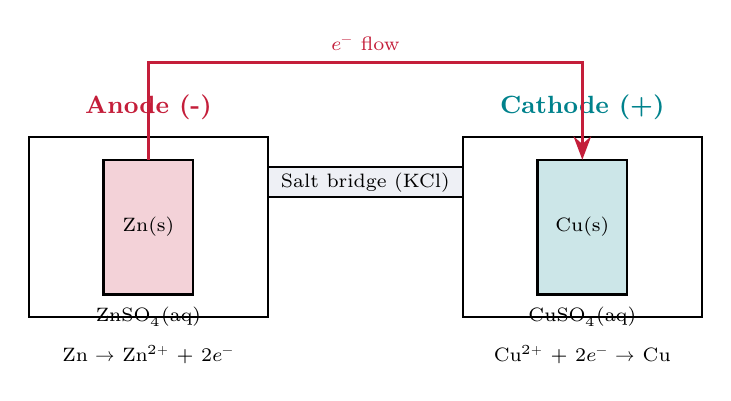
\begin{tikzpicture}[scale=0.95, node distance=0.3cm and 0.5cm,
  sblock/.style={rectangle, draw=myteal, fill=hdrteal, text width=2.0cm,
    align=center, minimum height=1.0cm, font=\small, rounded corners=3pt}]
  % Anode beaker
  \draw[thick] (0,0) rectangle (3.2,2.4);
  \node[font=\small\bfseries, color=myred] at (1.6,2.8) {Anode (-)};
  \draw[fill=myred!20, thick] (1.0,0.3) rectangle (2.2,2.1);
  \node[font=\scriptsize] at (1.6,1.2) {Zn(s)};
  \node[font=\scriptsize] at (1.6,0.0) {ZnSO$_4$(aq)};
  % Cathode beaker
  \draw[thick] (5.8,0) rectangle (9.0,2.4);
  \node[font=\small\bfseries, color=myteal] at (7.4,2.8) {Cathode (+)};
  \draw[fill=myteal!20, thick] (6.8,0.3) rectangle (8.0,2.1);
  \node[font=\scriptsize] at (7.4,1.2) {Cu(s)};
  \node[font=\scriptsize] at (7.4,0.0) {CuSO$_4$(aq)};
  % Salt bridge
  \draw[fill=hdrgray, thick] (3.2,1.6) rectangle (5.8,2.0);
  \node[font=\scriptsize] at (4.5,1.8) {Salt bridge (KCl)};
  % Electron flow (wire)
  \draw[redarrow, very thick] (1.6,2.1) -- (1.6,3.4) -- (7.4,3.4) -- (7.4,2.1);
  \node[font=\scriptsize, color=myred] at (4.5,3.65) {$e^-$ flow};
  % Half-reactions
  \node[font=\scriptsize, align=center] at (1.6,-0.5) {Zn $\to$ Zn$^{2+}$ + 2$e^-$};
  \node[font=\scriptsize, align=center] at (7.4,-0.5) {Cu$^{2+}$ + 2$e^-$ $\to$ Cu};
\end{tikzpicture}
\end{tcolorbox}

\subsection{Relationship Between \texorpdfstring{$\Delta G$}{Delta G} and Cell EMF}
\begin{tcolorbox}[formulabox, title={Free Energy and EMF}]
\[
\Delta G = -nFE, \qquad \Delta G^\circ = -nFE^\circ
\]
$n$ = number of electrons transferred; $F = 96485\ \mathrm{C\,mol^{-1}}$ (Faraday constant).\\
Combining with $\Delta G^\circ = -RT\ln K$:
\[
E^\circ = \frac{RT}{nF}\ln K = \frac{0.0257}{n}\ln K = \frac{0.0591}{n}\log K \quad (298\ \mathrm{K})
\]
\end{tcolorbox}

\subsection{Derivation of the Nernst Equation}
Starting from $\Delta G = \Delta G^\circ + RT\ln Q$ and substituting $\Delta G = -nFE$ and $\Delta G^\circ = -nFE^\circ$:
\[
-nFE = -nFE^\circ + RT\ln Q
\]
Dividing by $-nF$:

\begin{tcolorbox}[formulabox, title={Nernst Equation}]
\[
E = E^\circ - \frac{RT}{nF}\ln Q = E^\circ - \frac{0.0591}{n}\log Q \quad (298\ \mathrm{K})
\]
At equilibrium, $E = 0$ and $Q = K$, confirming $E^\circ = (0.0591/n)\log K$.
\end{tcolorbox}

\begin{tcolorbox}[examplebox, title={Solved Example: Daniell Cell EMF via Nernst}]
Zn/Cu cell: $E^\circ_{\mathrm{cell}} = 0.34 - (-0.76) = 1.10\ \mathrm{V}$, $n=2$.
If $[\mathrm{Zn^{2+}}] = 0.10\ \mathrm{M}$ and $[\mathrm{Cu^{2+}}] = 2.0\ \mathrm{M}$:
\[
Q = \frac{[\mathrm{Zn^{2+}}]}{[\mathrm{Cu^{2+}}]} = \frac{0.10}{2.0} = 0.050
\]
\[
E = 1.10 - \frac{0.0591}{2}\log(0.050) = 1.10 - 0.02955\times(-1.301) = 1.10 + 0.038 = 1.138\ \mathrm{V}
\]
Lower $[\mathrm{Zn^{2+}}]$ and higher $[\mathrm{Cu^{2+}}]$ increases the driving force above the standard value.
\end{tcolorbox}

\begin{tcolorbox}[examplebox, title={Solved Example: Equilibrium Constant from \texorpdfstring{$E^\circ$}{E0}}]
For the Daniell cell ($E^\circ = 1.10\ \mathrm{V}$, $n=2$):
\[
\log K = \frac{n\,E^\circ}{0.0591} = \frac{2\times1.10}{0.0591} = 37.23
\]
\[
K = 10^{37.23} \approx 1.7\times10^{37}
\]
An enormous $K$ confirms the reaction is essentially complete under standard conditions.
\end{tcolorbox}

\subsection{Concentration Cell}
A concentration cell uses the same electrode material in solutions of different concentrations. The EMF arises purely from the concentration difference.

\begin{tcolorbox}[formulabox, title={Concentration Cell EMF}]
\[
E = \frac{0.0591}{n}\log\frac{C_{\mathrm{high}}}{C_{\mathrm{low}}}
\]
At equal concentrations $E = 0$; the cell drives ions from high to low concentration.
\end{tcolorbox}

\subsection{Cell Notation and Standard Cell Notation}
Cells are written with the anode on the left and cathode on the right, separated by a double vertical line (salt bridge):
\[
\mathrm{Zn(s)}\;|\;\mathrm{Zn^{2+}(aq)}\;\|\;\mathrm{Cu^{2+}(aq)}\;|\;\mathrm{Cu(s)}
\]
Single vertical line $|$ = phase boundary; double $\|$ = salt bridge.\\
$E^\circ_{\mathrm{cell}} = E^\circ(\text{right half-cell}) - E^\circ(\text{left half-cell}) = 0.34 - (-0.76) = 1.10\ \mathrm{V}$.

\subsection{Fuel Cells}
A fuel cell is a galvanic device that converts the chemical energy of a fuel (usually H$_2$) directly to electricity without combustion.

\begin{tcolorbox}[formulabox, title={Hydrogen--Oxygen Fuel Cell Reactions}]
\textbf{Anode (alkaline medium):}\quad $\mathrm{2H_2 + 4OH^- \to 4H_2O + 4e^-}$\\
\textbf{Cathode:}\quad $\mathrm{O_2 + 2H_2O + 4e^- \to 4OH^-}$\\
\textbf{Overall:}\quad $\mathrm{2H_2 + O_2 \to 2H_2O}$,\quad $\Delta G^\circ = -474\ \mathrm{kJ\,mol^{-1}}$,\quad $E^\circ = 1.23\ \mathrm{V}$
\end{tcolorbox}

\textbf{Advantages of fuel cells over heat engines:}
\begin{itemize}[leftmargin=*, itemsep=1pt, topsep=2pt]
  \item Efficiency not limited by Carnot efficiency ($\eta_{\mathrm{max}} = 1-T_c/T_h$); can exceed 60\%.
  \item No moving parts in the electrochemical stack.
  \item Zero local emissions (H$_2$-O$_2$ cell produces only water).
  \item Used in spacecraft, buses, and stationary power plants.
\end{itemize}

\begin{tcolorbox}[exambox, title={Exam Points (Section 4)}]
\begin{itemize}[leftmargin=*, itemsep=2pt, topsep=2pt]
  \item $E^\circ_{\mathrm{cell}} = E^\circ_{\mathrm{cathode}} - E^\circ_{\mathrm{anode}}$; higher $E^\circ$ is cathode.
  \item $\Delta G = -nFE$; $\Delta G < 0$ when $E > 0$ (spontaneous cell).
  \item Derive Nernst from $\Delta G = \Delta G^\circ + RT\ln Q$.
  \item $\log K = n E^\circ / 0.0591$ at 298 K.
  \item Concentration cell: EMF from $\log(C_{\mathrm{high}}/C_{\mathrm{low}})$; same electrodes.
\end{itemize}
\end{tcolorbox}

% ===============================================================================
\section{Acid--Base, Redox, and Solubility Equilibria}
% ===============================================================================

\begin{tcolorbox}[defbox]
Three categories of aqueous equilibria are central to engineering chemistry: (i) acid--base equilibria (proton transfer), (ii) redox equilibria (electron transfer), and (iii) solubility equilibria (precipitation). All three are governed by $\Delta G^\circ = -RT\ln K$.
\end{tcolorbox}

\subsection{Br\o{}nsted--Lowry Acid--Base Theory}
\begin{tcolorbox}[defbox]
A \textbf{Br\o{}nsted--Lowry acid} donates a proton; a \textbf{base} accepts one. Every acid has a conjugate base (formed after proton loss) and every base has a conjugate acid. This theory covers aqueous and non-aqueous systems, unlike Arrhenius theory.
\end{tcolorbox}

\textbf{Water autoionisation:} $\mathrm{H_2O + H_2O \rightleftharpoons H_3O^+ + OH^-}$; $K_w = [\mathrm{H_3O^+}][\mathrm{OH^-}] = 1.0\times10^{-14}$ at 298 K.\\
$\mathrm{pH} + \mathrm{pOH} = 14$ at 298 K.

\subsection{Weak Acid Equilibrium and pH Derivation}
For a weak acid HA in water:
\[
\mathrm{HA} \rightleftharpoons \mathrm{H^+} + \mathrm{A^-}, \qquad K_a = \frac{[\mathrm{H^+}][\mathrm{A^-}]}{[\mathrm{HA}]}
\]
If initial concentration is $C$ and degree of dissociation $\alpha \ll 1$:
\[
[\mathrm{H^+}] = \sqrt{K_a C}, \qquad \mathrm{pH} = \tfrac{1}{2}(\mathrm{p}K_a - \log C)
\]

\begin{tcolorbox}[examplebox, title={Solved Example: pH of Acetic Acid}]
$0.10\ \mathrm{M}$ acetic acid, $K_a = 1.8\times10^{-5}$:
\[
[\mathrm{H^+}] = \sqrt{1.8\times10^{-5}\times0.10} = \sqrt{1.8\times10^{-6}} = 1.34\times10^{-3}\ \mathrm{M}
\]
\[
\mathrm{pH} = -\log(1.34\times10^{-3}) = 2.87
\]
Verify with formula: $\mathrm{pH} = \tfrac12(4.74 - (-1)) = 2.87$. \checkmark
\end{tcolorbox}

\subsection{Henderson--Hasselbalch Equation and Buffers}
A buffer solution resists pH change. It consists of a weak acid and its conjugate base (or weak base and conjugate acid).

\begin{tcolorbox}[formulabox, title={Henderson--Hasselbalch Equation}]
\[
\mathrm{pH} = \mathrm{p}K_a + \log\frac{[\mathrm{A^-}]}{[\mathrm{HA}]} = \mathrm{p}K_a + \log\frac{[\text{salt}]}{[\text{acid}]}
\]
\textbf{Derivation:} Take $-\log$ of $K_a = [\mathrm{H^+}][\mathrm{A^-}]/[\mathrm{HA}]$: $\mathrm{pK_a} = \mathrm{pH} - \log([\mathrm{A^-}]/[\mathrm{HA}])$; rearrange.\\
Buffer capacity is maximum when $[\mathrm{A^-}] = [\mathrm{HA}]$, i.e.\ $\mathrm{pH} = \mathrm{p}K_a$.
\end{tcolorbox}

\begin{tcolorbox}[examplebox, title={Solved Example: Buffer pH and Its Change on Adding Acid}]
Acetate buffer: $[\mathrm{CH_3COOH}] = 0.20\ \mathrm{M}$, $[\mathrm{CH_3COONa}] = 0.30\ \mathrm{M}$, $\mathrm{p}K_a = 4.74$:
\[
\mathrm{pH} = 4.74 + \log\frac{0.30}{0.20} = 4.74 + 0.18 = 4.92
\]
Adding $0.01\ \mathrm{mol}$ HCl to 1 L: acid consumes $0.01\ \mathrm{mol}$ of $\mathrm{CH_3COO^-}$:
\[
[\mathrm{A^-}] = 0.29\ \mathrm{M},\quad [\mathrm{HA}] = 0.21\ \mathrm{M},\quad
\mathrm{pH} = 4.74 + \log\frac{0.29}{0.21} = 4.74 + 0.14 = 4.88
\]
pH changed by only $0.04$ despite adding strong acid --- the buffer works.
\end{tcolorbox}

\subsection{Biological Importance of Buffers}
\begin{itemize}[leftmargin=*, itemsep=2pt, topsep=2pt]
  \item Blood pH ($7.35$--$7.45$) maintained by the bicarbonate buffer: $\mathrm{H_2CO_3}/\mathrm{HCO_3^-}$ ($\mathrm{p}K_a = 6.35$) reinforced by respiratory control of $\mathrm{CO_2}$.
  \item Intracellular pH maintained by phosphate buffer ($\mathrm{H_2PO_4^-}/\mathrm{HPO_4^{2-}}$, $\mathrm{p}K_a = 7.2$).
  \item Industrial buffers: electroplating baths, pharmaceutical formulations.
\end{itemize}

\subsection{Lewis Acid--Base Theory}
\begin{tcolorbox}[defbox]
\textbf{Lewis acid:} Electron-pair acceptor. \textbf{Lewis base:} Electron-pair donor. This is the broadest acid--base definition and covers reactions without proton transfer, such as complex-ion formation.
\end{tcolorbox}

\begin{tabularx}{\linewidth}{|B{2.4cm}|Y|Y|}
\hline
\textbf{Concept} & \textbf{Arrhenius} & \textbf{Brønsted--Lowry} and \textbf{Lewis} \\
\hline
Acid & Produces H$^+$ in water & H$^+$ donor / electron-pair acceptor \\
\hline
Base & Produces OH$^-$ in water & H$^+$ acceptor / electron-pair donor \\
\hline
Scope & Aqueous only & Aqueous and non-aqueous \\
\hline
Example & HCl, NaOH & NH$_3$: Lewis base; BF$_3$: Lewis acid \\
\hline
\end{tabularx}

\textbf{Lewis examples:} $\mathrm{BF_3 + NH_3 \to F_3B{:}NH_3}$ (adduct); metal-ligand complex formation $\mathrm{Cu^{2+} + 4NH_3 \to [Cu(NH_3)_4]^{2+}}$ (Cu$^{2+}$ = Lewis acid, NH$_3$ = Lewis base).

\subsection{Redox Equilibria and Disproportionation}
\begin{tcolorbox}[defbox]
\textbf{Disproportionation:} A reaction in which the same element is simultaneously oxidised and reduced. Example: $\mathrm{2Cu^+(aq) \to Cu^{2+}(aq) + Cu(s)}$.
\end{tcolorbox}

\textbf{Predicting feasibility of redox reactions using $E^\circ$:}
\begin{itemize}[leftmargin=*, itemsep=1pt, topsep=2pt]
  \item $E^\circ_{\mathrm{cell}} > 0$ ($\Delta G^\circ < 0$): reaction spontaneous.
  \item $E^\circ_{\mathrm{cell}} < 0$: non-spontaneous in the written direction.
\end{itemize}

\textbf{Disproportionation of Cu$^+$:}
\begin{align*}
\text{Cathode:}&\quad \mathrm{Cu^+(aq) + e^- \to Cu(s)},\quad E^\circ = +0.52\ \mathrm{V}\\
\text{Anode:}&\quad \mathrm{Cu(s) \to Cu^+(aq) + e^-},\quad E^\circ = -0.34\ \mathrm{V}\quad\text{wait...}
\end{align*}
Actually using the two half-reactions:
$\mathrm{Cu^+ + e^- \to Cu}$ ($+0.52\ \mathrm{V}$) and $\mathrm{Cu^{2+} + e^- \to Cu^+}$ ($+0.16\ \mathrm{V}$).
$E^\circ_{\mathrm{cell}} = 0.52 - 0.16 = +0.36\ \mathrm{V} > 0$, so Cu$^+$ is unstable to disproportionation in aqueous solution.

\subsection{Solubility Product \texorpdfstring{$K_{sp}$}{Ksp}}
For a sparingly soluble salt $\mathrm{M}_m\mathrm{X}_n(s) \rightleftharpoons m\mathrm{M}^{n+} + n\mathrm{X}^{m-}$:

\begin{tcolorbox}[formulabox, title={Solubility Product}]
\[
K_{sp} = [\mathrm{M}^{n+}]^m[\mathrm{X}^{m-}]^n
\]
\textbf{Ionic product (IP):} $[\mathrm{M}^{n+}]^m[\mathrm{X}^{m-}]^n$ using current concentrations.
\begin{itemize}[leftmargin=*, itemsep=1pt, topsep=2pt]
  \item IP $< K_{sp}$: unsaturated, no precipitation.
  \item IP $= K_{sp}$: saturated, equilibrium.
  \item IP $> K_{sp}$: supersaturated, precipitation occurs.
\end{itemize}
\end{tcolorbox}

\begin{tcolorbox}[examplebox, title={Solved Example: Solubility from \texorpdfstring{$K_{sp}$}{Ksp}}]
$K_{sp}(\mathrm{BaSO_4}) = 1.1\times10^{-10}$ at 298 K. Find molar solubility $s$ in pure water.
\[
\mathrm{BaSO_4 \rightleftharpoons Ba^{2+} + SO_4^{2-}},\quad K_{sp} = s\cdot s = s^2
\]
\[
s = \sqrt{1.1\times10^{-10}} = 1.05\times10^{-5}\ \mathrm{mol\,L^{-1}}
\]
In $0.10\ \mathrm{M}\ \mathrm{Na_2SO_4}$ (common ion effect):
\[
K_{sp} = s\cdot(0.10 + s) \approx 0.10\,s \quad\Rightarrow\quad s = \frac{1.1\times10^{-10}}{0.10} = 1.1\times10^{-9}\ \mathrm{mol\,L^{-1}}
\]
Common ion reduces solubility by a factor of $\sim 10^4$.
\end{tcolorbox}

\begin{tcolorbox}[exambox, title={Exam Points (Section 5)}]
\begin{itemize}[leftmargin=*, itemsep=2pt, topsep=2pt]
  \item Brønsted--Lowry: acid = proton donor; base = proton acceptor.
  \item $K_a \times K_b = K_w = 10^{-14}$; $\mathrm{pH + pOH = 14}$ at 298 K.
  \item Weak acid pH: $\mathrm{pH} = \tfrac12(\mathrm{pK_a} - \log C)$.
  \item Henderson--Hasselbalch: $\mathrm{pH} = \mathrm{pK_a} + \log([\mathrm{A^-}]/[\mathrm{HA}])$; buffer works near $\mathrm{pK_a}$.
  \item $K_{sp}$ solubility product: IP $> K_{sp}$ gives precipitation; common ion reduces solubility.
\end{itemize}
\end{tcolorbox}

% ===============================================================================
\section{Water Chemistry and Corrosion}
% ===============================================================================

\begin{tcolorbox}[defbox]
\textbf{Water chemistry} deals with the dissolved ions, gases, and organic matter in natural and industrial water, especially as they affect engineering systems. \textbf{Corrosion} is the electrochemical deterioration of metals driven by a spontaneous redox reaction ($\Delta G < 0$). Both topics are directly governed by the free-energy and equilibrium principles of this module.
\end{tcolorbox}

\subsection{Hardness of Water}
Hard water contains dissolved $\mathrm{Ca^{2+}}$ and $\mathrm{Mg^{2+}}$ ions, primarily as bicarbonates, chlorides, and sulphates. Hardness is expressed in parts per million (ppm) as equivalent $\mathrm{CaCO_3}$.

\begin{tcolorbox}[formulabox, title={Hardness in ppm as \texorpdfstring{$\mathrm{CaCO_3}$}{CaCO3} Equivalent}]
\[
\text{Hardness (ppm)} = \frac{\text{mass of salt (g)}}{\text{volume of water (L)}}\times\frac{M(\mathrm{CaCO_3})}{M(\text{salt})}\times1000
\]
Or: $\text{ppm} = \frac{w_{\mathrm{CaCO_3\text{-equiv}}}}{V_{\text{water}}}\times10^6$.\\
Soft water: $<75\ \mathrm{ppm}$. Moderately hard: $75$--$150\ \mathrm{ppm}$. Hard: $>150\ \mathrm{ppm}$.
\end{tcolorbox}

\begin{tabularx}{\linewidth}{|B{2.8cm}|Y|Y|}
\hline
\textbf{Type} & \textbf{Cause} & \textbf{Removal} \\
\hline
Temporary hardness & $\mathrm{Ca(HCO_3)_2}$, $\mathrm{Mg(HCO_3)_2}$ & Boiling, lime addition \\
\hline
Permanent hardness & $\mathrm{CaCl_2}$, $\mathrm{MgCl_2}$, $\mathrm{CaSO_4}$, $\mathrm{MgSO_4}$ & Lime-soda, zeolite, ion exchange \\
\hline
\end{tabularx}

\subsection{Boiler Troubles}
Hard water in steam boilers causes multiple engineering problems.

\begin{tabularx}{\linewidth}{|B{2.6cm}|Y|Y|Y|}
\hline
\textbf{Problem} & \textbf{Cause} & \textbf{Effect} & \textbf{Remedy} \\
\hline
Scale formation & Deposition of $\mathrm{CaCO_3}$, $\mathrm{Mg(OH)_2}$, $\mathrm{CaSO_4}$ & Reduced heat transfer; tube overheating and bursting & Softening; acid descaling \\
\hline
Sludge formation & Loose precipitates of $\mathrm{MgCO_3}$, $\mathrm{MgCl_2}$ & Chokes pipes; reduces efficiency & Blow-down of boiler \\
\hline
Priming & High dissolved solids, oil, or organic impurities & Wet steam carries water droplets; turbine erosion & Filtration; demineralisation \\
\hline
Foaming & Organic impurities or oil stabilise steam bubbles & Irregular operation; carryover & Anti-foam chemicals \\
\hline
Caustic embrittlement & Concentrated NaOH in stressed joints/cracks & Metal grain-boundary cracking and failure & Neutralise with sodium sulphate \\
\hline
\end{tabularx}

\subsection{Water Softening Methods}
\begin{tabularx}{\linewidth}{|B{2.6cm}|Y|Y|}
\hline
\textbf{Method} & \textbf{Principle} & \textbf{Notes} \\
\hline
Lime--soda process & Add $\mathrm{Ca(OH)_2}$ and $\mathrm{Na_2CO_3}$; precipitate $\mathrm{CaCO_3}$ and $\mathrm{Mg(OH)_2}$ & Cheap; used for large volumes; produces sludge \\
\hline
Zeolite / ion exchange & $\mathrm{Ca^{2+}}$ and $\mathrm{Mg^{2+}}$ exchanged for $\mathrm{Na^+}$ on zeolite resin & Portable; regenerated with NaCl; does not reduce TDS \\
\hline
Demineralisation & Cation exchanger (H$^+$ form) + anion exchanger (OH$^-$ form) & Removes all ions; produces ultra-pure water \\
\hline
Reverse osmosis & Applied pressure forces water through semi-permeable membrane & Removes ions, bacteria, organics \\
\hline
\end{tabularx}

\subsection{Electrochemical Theory of Corrosion}
Corrosion of iron in neutral or acidic water is an electrochemical process requiring an anode (oxidation), a cathode (reduction), an electrolyte, and a metallic conductor.

\begin{tcolorbox}[formulabox, title={Iron Corrosion Half-Reactions}]
\textbf{Anodic reaction (oxidation):}
\[
\mathrm{Fe(s) \to Fe^{2+}(aq) + 2e^-}, \qquad E^\circ = +0.44\ \mathrm{V\ (vs\ SHE)}
\]
\textbf{Cathodic reaction (oxygen reduction, neutral/alkaline):}
\[
\mathrm{O_2(g) + 2H_2O(l) + 4e^- \to 4OH^-(aq)}, \qquad E^\circ = +0.40\ \mathrm{V}
\]
\textbf{Overall:}
\[
\mathrm{2Fe + O_2 + 2H_2O \to 2Fe(OH)_2}
\]
Further air oxidation: $\mathrm{4Fe(OH)_2 + O_2 + 2H_2O \to 4Fe(OH)_3}$ $\to$ rust (hydrated $\mathrm{Fe_2O_3}$).
\end{tcolorbox}

\begin{tcolorbox}[tikzbox, title={Differential Aeration Corrosion Cell}]
\centering
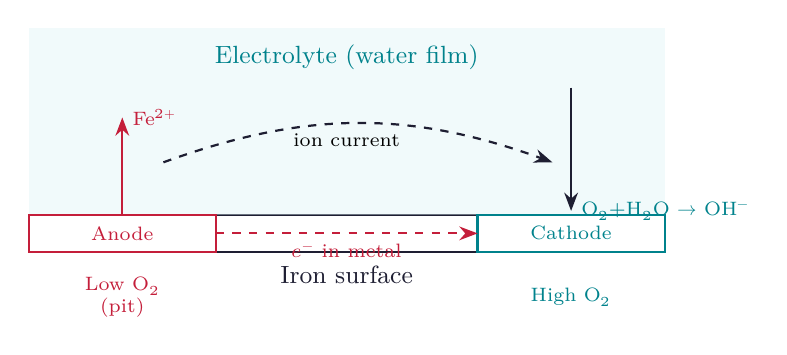
\begin{tikzpicture}[scale=0.95]
  % Iron surface
  \draw[thick, mydark] (0,0) rectangle (8.5,0.5);
  \node[font=\small, color=mydark] at (4.25,-0.3) {Iron surface};
  % Electrolyte above
  \fill[hdrteal, opacity=0.4] (0,0.5) rectangle (8.5,3.0);
  \node[font=\small, color=myteal] at (4.25,2.6) {Electrolyte (water film)};
  % Anode region (left, low O2)
  \draw[thick, myred] (0,0) rectangle (2.5,0.5);
  \node[font=\scriptsize, color=myred] at (1.25,0.25) {Anode};
  \node[font=\scriptsize, color=myred, align=center] at (1.25,-0.6) {Low O$_2$\\(pit)};
  \draw[redarrow] (1.25,0.5) -- (1.25,1.8) node[right, font=\scriptsize, color=myred] {Fe$^{2+}$};
  % Cathode region (right, high O2)
  \draw[thick, myteal] (6.0,0) rectangle (8.5,0.5);
  \node[font=\scriptsize, color=myteal] at (7.25,0.25) {Cathode};
  \node[font=\scriptsize, color=myteal, align=center] at (7.25,-0.6) {High O$_2$};
  \draw[arrow] (7.25,2.2) -- (7.25,0.55) node[right, font=\scriptsize, color=myteal] {O$_2$+H$_2$O $\to$ OH$^-$};
  % Electron flow in metal
  \draw[redarrow, dashed] (2.5,0.25) -- (6.0,0.25) node[midway, below, font=\scriptsize] {$e^-$ in metal};
  % Ion flow in electrolyte
  \draw[arrow, dashed] (1.8,1.2) to[bend left=20] (7.0,1.2);
  \node[font=\scriptsize] at (4.25,1.5) {ion current};
\end{tikzpicture}
\end{tcolorbox}

\textbf{Factors accelerating corrosion:} Higher temperature, lower pH, higher dissolved $\mathrm{O_2}$, electrolyte concentration, stressed metal, galvanic coupling with nobler metal.

\subsection{Dissolved Oxygen, BOD, and COD}
These three parameters are standard measures of water quality and appear in MAKAUT water-chemistry questions.

\begin{tcolorbox}[defbox]
\textbf{Dissolved Oxygen (DO):} Oxygen dissolved in water; typical freshwater has $8$--$14\ \mathrm{mg\,L^{-1}}$. Falls below $5\ \mathrm{mg\,L^{-1}}$ in polluted water, harming aquatic life.\\
\textbf{BOD (Biochemical Oxygen Demand):} Oxygen consumed by microorganisms to decompose organic matter in 5 days at 20$^\circ$C (BOD$_5$). High BOD = heavy organic pollution.\\
\textbf{COD (Chemical Oxygen Demand):} Oxygen equivalent needed to oxidise all organic and inorganic matter chemically (with K$_2$Cr$_2$O$_7$ as oxidant). COD $\geq$ BOD always.
\end{tcolorbox}

\begin{tabularx}{\linewidth}{|B{2.6cm}|Y|Y|}
\hline
\textbf{Parameter} & \textbf{Clean water} & \textbf{Polluted water} \\
\hline
DO (mg/L) & 8--14 & $<$5 (danger zone) \\
\hline
BOD (mg/L) & $<$1--2 & $>$100 (sewage $\sim$ 300) \\
\hline
COD (mg/L) & $<$10 & $>$150 \\
\hline
\end{tabularx}

\subsection{Passivation}
\begin{tcolorbox}[defbox]
\textbf{Passivation:} Formation of a thin, dense, adherent oxide film on a metal surface that blocks further corrosion. The film is self-healing when scratched in air. Examples: Al forms Al$_2$O$_3$ (3 nm thick), stainless steel forms Cr$_2$O$_3$, Ti forms TiO$_2$.
\end{tcolorbox}

Passivation requires the oxide to be: (i) insoluble in the corrosive medium, (ii) adherent (not flaking), (iii) dense enough to prevent ion/electron diffusion.\\
\textbf{Concentration of HNO$_3$ and passivation of iron:} Dilute HNO$_3$ dissolves iron (active dissolution); concentrated HNO$_3$ passivates iron by forming a dense Fe$_3$O$_4$/Fe$_2$O$_3$ surface layer — a standard MAKAUT viva question.

\subsection{Corrosion Prevention}
\begin{tabularx}{\linewidth}{|B{2.8cm}|Y|Y|}
\hline
\textbf{Method} & \textbf{Principle} & \textbf{Example} \\
\hline
Barrier coatings & Physically isolate metal from electrolyte & Paint, polymer coating, oxide passivation \\
\hline
Galvanisation & Sacrificial zinc oxidises preferentially to iron; even at scratches Zn protects Fe & Zn-coated steel sheets \\
\hline
Sacrificial anode & More active metal (Mg, Zn, Al) connected as anode; made to corrode instead of structure & Ship hulls, buried pipelines \\
\hline
Impressed current & External DC supply makes structure cathodic; no net oxidation & Underground pipelines, bridges \\
\hline
Alloying & Cr$_2$O$_3$ passive film on stainless steel blocks O$_2$/H$_2$O access & Stainless steel ($>11\%$ Cr) \\
\hline
Inhibitors & Adsorb on metal surface, reduce anodic/cathodic reaction rate & Boiler treatment chemicals \\
\hline
\end{tabularx}

\textbf{Sacrificial anode vs impressed current:}\par\noindent
\begin{tabularx}{\linewidth}{|B{3.0cm}|Y|Y|}
\hline
\textbf{Feature} & \textbf{Sacrificial anode} & \textbf{Impressed current} \\
\hline
Power source & None (galvanic cell) & External DC rectifier \\
\hline
Anode material & Mg, Zn, or Al alloy & Inert (platinised Ti, graphite) \\
\hline
Maintenance & Replace anode periodically & Monitor current; less material cost \\
\hline
Suitable for & Small isolated structures & Large structures, long pipelines \\
\hline
\end{tabularx}

\begin{tcolorbox}[exambox, title={Exam Points (Section 6)}]
\begin{itemize}[leftmargin=*, itemsep=2pt, topsep=2pt]
  \item Hardness ppm = mass of CaCO$_3$ equivalent per litre $\times 10^6$.
  \item Temporary hardness: bicarbonates; removed by boiling. Permanent: chlorides/sulphates; need chemical treatment.
  \item Boiler scale: CaCO$_3$ and CaSO$_4$ deposits reduce heat transfer and cause overheating.
  \item Corrosion: Fe is anode (oxidised); O$_2$/H$^+$ cathodic reduction drives current.
  \item Sacrificial anode: Zn/Mg corrodes preferentially protecting Fe.
  \item Stainless steel: passive Cr$_2$O$_3$ film blocks electrolyte contact.
\end{itemize}
\end{tcolorbox}

% ===============================================================================
\section{Ellingham Diagrams and Free Energy in Metallurgy}
% ===============================================================================

\begin{tcolorbox}[defbox]
An \textbf{Ellingham diagram} plots the standard Gibbs free energy of oxide formation ($\Delta G^\circ = \Delta H^\circ - T\Delta S^\circ$) against temperature for a series of metal--oxygen reactions. It is the primary tool for selecting a reducing agent in pyrometallurgy and for predicting the stability of oxides.
\end{tcolorbox}

\subsection{Construction and Interpretation}
For the standard reaction written as oxidation of 1 mol O$_2$:
\[
\tfrac{2x}{y}\mathrm{M}(s) + \mathrm{O_2}(g) \to \tfrac{2}{y}\mathrm{M_xO_y}(s)
\]
$\Delta G^\circ = \Delta H^\circ - T\Delta S^\circ$.

\begin{itemize}[leftmargin=*, itemsep=2pt, topsep=2pt]
  \item Mostly straight lines because $\Delta H^\circ$ and $\Delta S^\circ$ are nearly independent of $T$.
  \item Slope $= -\Delta S^\circ_{\mathrm{rxn}}$. Consuming one mole O$_2$(g) makes $\Delta S^\circ < 0$ (gas disappears), so slope is \emph{positive} (line rises with $T$) for most metal oxidations.
  \item \textbf{Exceptions:} $\mathrm{C + O_2 \to CO_2}$: $\Delta n_{\mathrm{gas}} = 0$, nearly horizontal. $\mathrm{2C + O_2 \to 2CO}$: $\Delta n_{\mathrm{gas}} = +1$, slope is \emph{negative} (line falls with $T$).
  \item \textbf{Slope changes:} A kink (sudden change in slope) occurs at the melting or boiling point of the metal because $\Delta S^\circ$ changes (latent heat term).
\end{itemize}

\begin{tcolorbox}[tikzbox, title={Schematic Ellingham Diagram (three key lines)}]
\centering
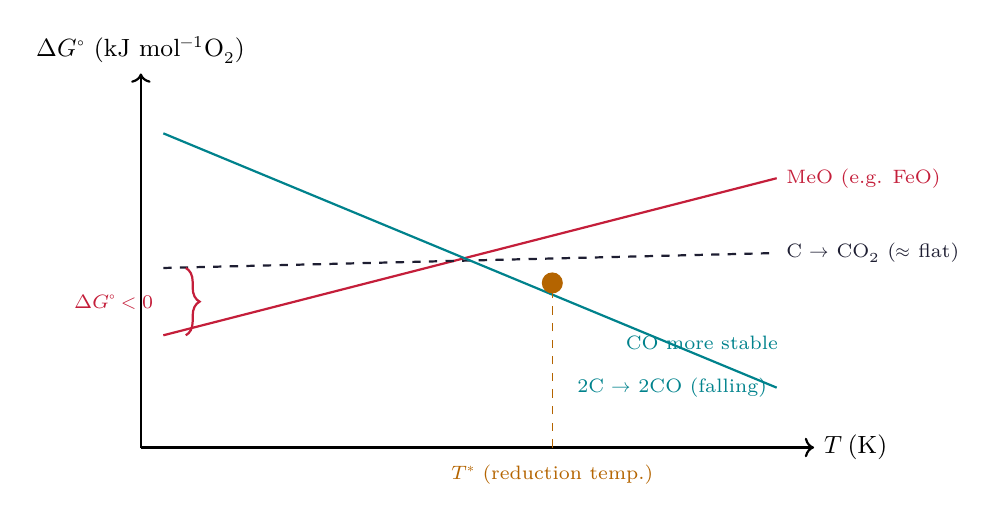
\begin{tikzpicture}[scale=0.95]
  \draw[->, thick] (0,0) -- (9.0,0) node[right, font=\small] {$T$ (K)};
  \draw[->, thick] (0,0) -- (0,5.0) node[above, font=\small] {$\Delta G^\circ$ (kJ mol$^{-1}$O$_2$)};
  % Metal oxide (rising line, e.g. Fe2O3)
  \draw[myred, thick] (0.3,1.5) -- (8.5,3.6);
  \node[myred, font=\scriptsize, anchor=west] at (8.5,3.6) {MeO (e.g. FeO)};
  % C -> CO2 (nearly horizontal)
  \draw[mydark, thick, dashed] (0.3,2.4) -- (8.5,2.6);
  \node[mydark, font=\scriptsize, anchor=west] at (8.5,2.6) {C $\to$ CO$_2$ ($\approx$ flat)};
  % 2C -> 2CO (falling line, crosses MeO at T*)
  \draw[myteal, thick] (0.3,4.2) -- (8.5,0.8);
  \node[myteal, font=\scriptsize, anchor=east] at (8.5,0.8) {2C $\to$ 2CO (falling)};
  % Crossover
  \fill[myamber] (5.5,2.2) circle (4pt);
  \draw[dashed, myamber] (5.5,0) -- (5.5,2.2);
  \node[myamber, font=\scriptsize, anchor=north] at (5.5,-0.1) {$T^*$ (reduction temp.)};
  % Arrow
  \draw[decorate, decoration={brace, amplitude=5pt}, myred, thick]
       (0.6,2.4) -- (0.6,1.5) node[midway, left=8pt, font=\scriptsize, color=myred] {$\Delta G^\circ < 0$};
  \node[font=\scriptsize, color=myteal] at (7.5,1.4) {CO more stable};
\end{tikzpicture}
\end{tcolorbox}

\subsection{Rules for Selecting a Reducing Agent}
\begin{tcolorbox}[formulabox, title={Ellingham Selection Rule}]
A metal oxide $\mathrm{MO}$ can be reduced by a reducing agent $\mathrm{R}$ at temperature $T$ if the $\Delta G^\circ$ line of $\mathrm{R+O_2 \to RO_2}$ lies \emph{below} the $\Delta G^\circ$ line of $\mathrm{2M+O_2 \to 2MO}$ at that temperature.

The overall reaction $\mathrm{MO + R \to M + RO}$ has $\Delta G^\circ = \Delta G^\circ(\mathrm{MO\;line}) - \Delta G^\circ(\mathrm{RO\;line}) > 0$ … wait --- actually \emph{subtract lower from upper}: net $\Delta G^\circ < 0$ only when the reducing agent's line is lower.

In short: \textbf{the oxide whose line is lower is more stable; its metal is harder to reduce. Use a reducing agent whose line is below the ore's line at the operating temperature.}
\end{tcolorbox}

\subsection{Carbon as a Reducing Agent: The Blast Furnace}
Carbon has two Ellingham lines: $\mathrm{C + O_2 \to CO_2}$ (flat) and $\mathrm{2C + O_2 \to 2CO}$ (descending). Above $\sim 700^\circ\mathrm{C}$ the CO line lies below most metal oxide lines, making carbon (via CO) an effective industrial reducing agent.

\textbf{Blast furnace reactions:}
\begin{align*}
\mathrm{C + O_2} &\to \mathrm{CO_2} \quad \text{(combustion zone)}\\
\mathrm{CO_2 + C} &\to \mathrm{2CO} \quad \text{(Boudouard reaction)}\\
\mathrm{Fe_2O_3 + 3CO} &\to \mathrm{2Fe + 3CO_2} \quad \text{(reduction zone)}\\
\mathrm{CaCO_3} &\to \mathrm{CaO + CO_2} \quad \text{(flux decomposition)}\\
\mathrm{CaO + SiO_2} &\to \mathrm{CaSiO_3} \quad \text{(slag formation)}
\end{align*}

\subsection{Thermite Reaction: Aluminium Reducing Iron Oxide}
Aluminium sits below iron oxide on the Ellingham diagram at room temperature, so:
\[
\mathrm{Fe_2O_3 + 2Al \to Al_2O_3 + 2Fe}, \qquad \Delta G^\circ \approx -842\ \mathrm{kJ\,mol^{-1}}
\]
The large negative $\Delta G^\circ$ means the reaction is strongly spontaneous and highly exothermic ($\Delta H \approx -847\ \mathrm{kJ\,mol^{-1}}$), producing liquid iron at $\sim 2500\ \mathrm{K}$. Used in rail welding and incendiary applications.

\begin{tcolorbox}[examplebox, title={Solved Example: Reading the Ellingham Diagram}]
\textbf{Problem:} At what minimum temperature can coke (carbon) reduce ZnO?\\
\textbf{Given:} The $\Delta G^\circ$ lines of $\mathrm{2Zn + O_2 \to 2ZnO}$ and $\mathrm{2C + O_2 \to 2CO}$ cross at approximately $T^* = 950^\circ\mathrm{C}$.
\[
\text{Above } 950^\circ\mathrm{C}: \quad \Delta G^\circ(\mathrm{C\to CO}) < \Delta G^\circ(\mathrm{Zn\to ZnO})
\]
\[
\mathrm{ZnO + C \to Zn + CO}, \qquad \Delta G^\circ_{\mathrm{net}} < 0
\]
Industrial zinc smelters operate at $\sim 1000$--$1100^\circ\mathrm{C}$.
\end{tcolorbox}

\subsection{Limitations of Ellingham Diagrams}
\begin{itemize}[leftmargin=*, itemsep=2pt, topsep=2pt]
  \item Assumes pure solid/liquid phases (unit activity); does not account for alloy formation.
  \item Does not give information about reaction rate (kinetics).
  \item Phase changes (melting, boiling) cause kinks but data is not always available for all phases.
  \item Atmospheric composition (partial pressure of O$_2$) affects actual $\Delta G$.
\end{itemize}

\subsection{Industrial Extraction Examples Using Ellingham Diagram}
\begin{tabularx}{\linewidth}{|B{2.4cm}|Y|Y|Y|}
\hline
\textbf{Metal} & \textbf{Ore} & \textbf{Reducing agent at $T$} & \textbf{Typical temperature} \\
\hline
Iron (Fe) & Fe$_2$O$_3$ (haematite) & C (as CO) in blast furnace & $800$--$1600^\circ$C \\
\hline
Copper (Cu) & Cu$_2$S (chalcocite) & Roasting to Cu$_2$O then C or self-reduction & $\sim 1000^\circ$C \\
\hline
Zinc (Zn) & ZnO (from roasting ZnS) & C (as CO/C) & $\sim 1000^\circ$C \\
\hline
Lead (Pb) & PbO (from roasting galena) & C & $\sim 700^\circ$C \\
\hline
Aluminium (Al) & Al$_2$O$_3$ (bauxite) & Electrolysis (too stable for C reduction) & Hall-H\'{e}roult at $960^\circ$C \\
\hline
\end{tabularx}

\textbf{Why aluminium cannot be reduced by carbon from Ellingham:} The Al$_2$O$_3$ line is always below the CO line even at 2000$^\circ$C. The reaction Al$_2$O$_3$ + C $\to$ Al + CO has $\Delta G^\circ > 0$ at all practical temperatures, so electrolysis is used instead.

\begin{tcolorbox}[exambox, title={Exam Points (Section 7)}]
\begin{itemize}[leftmargin=*, itemsep=2pt, topsep=2pt]
  \item Ellingham line slope = $-\Delta S^\circ$; positive (rising) for most metal oxidations; negative for $2\mathrm{C}\to2\mathrm{CO}$.
  \item Reducing agent selection: line below = more stable oxide = better reducing agent.
  \item Blast furnace: C converts to CO via Boudouard reaction; CO reduces Fe$_2$O$_3$ above $\sim700^\circ$C.
  \item Thermite: Al reduces Fe$_2$O$_3$; $\Delta G^\circ \approx -842\ \mathrm{kJ\,mol^{-1}}$.
  \item Kink in a line: phase change (melting/boiling of metal).
\end{itemize}
\end{tcolorbox}

\newpage
\begin{center}
  {\large\bfseries\color{myred} Quick Revision --- Module 4}\\[3pt]
  {\small\color{mydark} Free Energy and Chemical Equilibria $|$ BS-CH101}
\end{center}
\noindent{\color{myred}\rule{\linewidth}{1.2pt}}
\vspace{6pt}

% --- Key Formulas: longtable so it breaks cleanly across pages ---------------
\begin{tcolorbox}[formulabox, breakable, title={Key Formulas at a Glance},
  title after break={\textbf{Key Formulas at a Glance (contd.)}}]
\renewcommand{\arraystretch}{1.55}
\begin{tabularx}{\linewidth}{|B{4.6cm}|Y|}
\hline
\textbf{Formula} & \textbf{Meaning} \\
\hline
$\Delta U = q + w$ & First law: energy conserved. \\
\hline
$\Delta H = \Delta U + \Delta(PV)$ & Enthalpy; at const $P$: $q_P = \Delta H$. \\
\hline
$C_P - C_V = R$ & Ideal gas heat capacity relation. \\
\hline
$\Delta H_{\mathrm{rxn}} = \sum \Delta H_f^\circ(\text{prod}) - \sum \Delta H_f^\circ(\text{react})$ & Hess's law. \\
\hline
$\Delta S = \displaystyle\int \frac{\delta q_{\mathrm{rev}}}{T}$ & Entropy from reversible heat. \\
\hline
$\Delta S_{\mathrm{univ}} = \Delta S_{\mathrm{sys}} + \Delta S_{\mathrm{surr}} \geq 0$ & Second law. \\
\hline
$\Delta G = \Delta H - T\Delta S$ & Gibbs free energy criterion. \\
\hline
$T^* = \Delta H / \Delta S$ & Crossover temperature ($\Delta G = 0$). \\
\hline
\end{tabularx}
\vspace{3pt}
\begin{tabularx}{\linewidth}{|B{4.6cm}|Y|}
\hline
$\left(\displaystyle\frac{\partial(\Delta G/T)}{\partial T}\right)_P = -\displaystyle\frac{\Delta H}{T^2}$ & Gibbs--Helmholtz equation. \\
\hline
$\Delta G = \Delta G^\circ + RT\ln Q$ & Free energy at non-standard conditions. \\
\hline
$\Delta G^\circ = -RT\ln K$ & Standard free energy and equilibrium constant. \\
\hline
$\ln\displaystyle\frac{K_2}{K_1} = -\displaystyle\frac{\Delta H^\circ}{R}\!\left(\displaystyle\frac{1}{T_2}-\displaystyle\frac{1}{T_1}\right)$ & Van't Hoff equation. \\
\hline
$E^\circ_{\mathrm{cell}} = E^\circ_{\mathrm{cathode}} - E^\circ_{\mathrm{anode}}$ & Standard cell EMF. \\
\hline
$\Delta G = -nFE$;\; $\Delta G^\circ = -nFE^\circ$ & Free energy and EMF. \\
\hline
$E = E^\circ - \displaystyle\frac{0.0591}{n}\log Q$ & Nernst equation at 298 K. \\
\hline
$\log K = \displaystyle\frac{n E^\circ}{0.0591}$ & $K$ from standard cell EMF. \\
\hline
\end{tabularx}
\vspace{3pt}
\begin{tabularx}{\linewidth}{|B{4.6cm}|Y|}
\hline
$K_w = [\mathrm{H^+}][\mathrm{OH^-}] = 10^{-14}$ & Water ionic product (298 K). \\
\hline
$\mathrm{pH} = \tfrac12(\mathrm{pK_a} - \log C)$ & pH of weak acid solution. \\
\hline
$\mathrm{pH} = \mathrm{p}K_a + \log\displaystyle\frac{[\mathrm{A^-}]}{[\mathrm{HA}]}$ & Henderson--Hasselbalch (buffer). \\
\hline
$K_{sp} = [\mathrm{M}^{n+}]^m[\mathrm{X}^{m-}]^n$ & Solubility product. \\
\hline
$K_p = K_c\,(RT)^{\Delta n_g}$ & Relationship between $K_p$ and $K_c$. \\
\hline
$w_{\mathrm{rev}} = -nRT\ln(V_2/V_1)$ & Reversible isothermal expansion work. \\
\hline
$\Delta S_{\mathrm{vap}} = \Delta H_{\mathrm{vap}}/T_b$ & Entropy of vaporisation. \\
\hline
$\Delta H_{T_2} = \Delta H_{T_1} + \Delta C_P\,(T_2-T_1)$ & Kirchhoff's equation. \\
\hline
$s = \sqrt{K_{sp}}$ & Molar solubility of 1:1 salt. \\
\hline
\end{tabularx}
\end{tcolorbox}

\begin{tcolorbox}[defbox, title={One-Line Definitions}]
\begin{itemize}[leftmargin=*, itemsep=2pt, topsep=2pt]
  \item \textbf{Internal energy ($U$):} Total kinetic and potential energy of all molecules in a system.
  \item \textbf{Enthalpy ($H$):} $H = U + PV$; heat flow at constant pressure.
  \item \textbf{Heat capacity ($C_P$):} Heat required to raise temperature by 1 K at constant pressure.
  \item \textbf{Hess's law:} Enthalpy change is independent of reaction pathway.
  \item \textbf{Entropy ($S$):} Measure of energy dispersal; $\Delta S_{\mathrm{univ}} > 0$ for spontaneous processes.
  \item \textbf{Third law:} $S = 0$ for a perfect crystal at $T = 0\ \mathrm{K}$.
  \item \textbf{Gibbs free energy ($G$):} $G = H - TS$; $\Delta G < 0$ for spontaneous process at const $T$, $P$.
  \item \textbf{Crossover temperature ($T^*$):} Temperature at which $\Delta G = 0$; $T^* = \Delta H/\Delta S$.
  \item \textbf{Reaction quotient ($Q$):} Ratio of product to reactant activities at current conditions.
  \item \textbf{Equilibrium constant ($K$):} $Q$ at equilibrium; $\Delta G^\circ = -RT\ln K$.
  \item \textbf{Van't Hoff equation:} Describes temperature dependence of $K$; derived from $\Delta G^\circ = \Delta H^\circ - T\Delta S^\circ$.
  \item \textbf{Le Chatelier's principle:} System shifts to partially counteract any imposed change.
  \item \textbf{Standard hydrogen electrode (SHE):} Reference electrode, $E^\circ = 0.000\ \mathrm{V}$.
  \item \textbf{Nernst equation:} $E = E^\circ - (RT/nF)\ln Q$; relates cell potential to concentration.
  \item \textbf{Faraday constant ($F$):} $96485\ \mathrm{C\,mol^{-1}}$; charge per mole of electrons.
  \item \textbf{Concentration cell:} Cell with identical electrodes at different concentrations; EMF from $\log(C_1/C_2)$.
  \item \textbf{Brønsted--Lowry acid:} Proton donor; its conjugate base forms after proton loss.
  \item \textbf{Buffer solution:} Resists pH change; contains weak acid + conjugate base near $\mathrm{pK_a}$.
  \item \textbf{Henderson--Hasselbalch:} $\mathrm{pH} = \mathrm{pK_a} + \log([\mathrm{A^-}]/[\mathrm{HA}])$.
  \item \textbf{Solubility product ($K_{sp}$):} Ion activity product in a saturated solution.
  \item \textbf{Common ion effect:} Adding a common ion suppresses solubility.
  \item \textbf{Temporary hardness:} Due to bicarbonates; removed by boiling.
  \item \textbf{Permanent hardness:} Due to chlorides/sulphates; requires chemical treatment.
  \item \textbf{Scale:} Hard insulating deposit in boilers; reduces heat transfer.
  \item \textbf{Galvanisation:} Coating iron with zinc; Zn acts as sacrificial anode.
  \item \textbf{Ellingham diagram:} $\Delta G^\circ$ vs $T$ plot for metal oxide formation; used to select reducing agents.
  \item \textbf{Passivation:} Dense oxide film that blocks further corrosion on a metal surface.
  \item \textbf{BOD:} Biochemical oxygen demand; oxygen consumed by microbes to decompose organics in 5 days at 20$^\circ$C.
  \item \textbf{COD:} Chemical oxygen demand; oxygen equivalent to oxidise all matter chemically; COD $\geq$ BOD.
  \item \textbf{Lewis acid:} Electron-pair acceptor (e.g.\ BF$_3$, metal ions).
  \item \textbf{Lewis base:} Electron-pair donor (e.g.\ NH$_3$, H$_2$O).
  \item \textbf{Disproportionation:} Same element simultaneously oxidised and reduced (e.g.\ 2Cu$^+ \to$ Cu + Cu$^{2+}$).
  \item \textbf{$K_p$ and $K_c$:} Related by $K_p = K_c(RT)^{\Delta n_g}$; equal when $\Delta n_g = 0$.
  \item \textbf{Kirchhoff's equation:} $\Delta H$ varies with temperature as $d(\Delta H)/dT = \Delta C_P$.
  \item \textbf{Trouton's rule:} $\Delta S_{\mathrm{vap}} \approx 85\ \mathrm{J\,mol^{-1}\,K^{-1}}$ for non-associated liquids at their normal boiling point.
\end{itemize}
\end{tcolorbox}

\begin{tcolorbox}[exambox, title={Frequently Asked / Viva Questions}]
\begin{enumerate}[topsep=0pt, label=\textbf{Q\arabic*.}, itemsep=5pt]
  \item \Q{State the first law of thermodynamics.}
    $\Delta U = q + w$; energy is conserved; heat and work are equivalent forms of energy transfer.
  \item \Q{What is enthalpy and why is it useful?}
    $H = U + PV$; at constant pressure, $\Delta H = q_P$ — directly measurable as heat flow in open experiments.
  \item \Q{State Hess's law with one example.}
    Enthalpy change is independent of pathway. Example: $\Delta H_{\mathrm{combustion}}$ of C to CO derived from $\Delta H$ of C $\to$ CO$_2$ and CO $\to$ CO$_2$.
  \item \Q{State the second law of thermodynamics.}
    For any spontaneous process, $\Delta S_{\mathrm{universe}} > 0$; for reversible processes $= 0$.
  \item \Q{What is Gibbs free energy and its spontaneity criterion?}
    $G = H - TS$; at constant $T$ and $P$: $\Delta G < 0$ spontaneous, $\Delta G = 0$ equilibrium, $\Delta G > 0$ non-spontaneous.
  \item \Q{List the four cases of $\Delta H$ and $\Delta S$ signs.}
    $(-,+)$: always spontaneous. $(+,-)$: never. $(-,-)$: spontaneous at low $T$. $(+,+)$: spontaneous at high $T$.
  \item \Q{Derive $\Delta G^\circ = -RT\ln K$.}
    At equilibrium, $\Delta G = 0$ and $Q = K$. Substituting in $\Delta G = \Delta G^\circ + RT\ln Q$ gives $0 = \Delta G^\circ + RT\ln K$, so $\Delta G^\circ = -RT\ln K$.
  \item \Q{State the van't Hoff equation.}
    $d\ln K/dT = \Delta H^\circ/(RT^2)$; exothermic reactions have $K$ decreasing with $T$.
  \item \Q{What is the Nernst equation?}
    $E = E^\circ - (RT/nF)\ln Q = E^\circ - (0.0591/n)\log Q$ at 298 K; it accounts for concentration effects on cell EMF.
  \item \Q{How is $K$ found from $E^\circ$?}
    $\log K = nE^\circ/0.0591$ at 298 K; derived from $\Delta G^\circ = -nFE^\circ = -RT\ln K$.
  \item \Q{What is a concentration cell?}
    Cell with same electrode in solutions of different concentrations; $E = (0.0591/n)\log(C_{\mathrm{high}}/C_{\mathrm{low}})$.
  \item \Q{What is the Henderson--Hasselbalch equation?}
    $\mathrm{pH} = \mathrm{pK_a} + \log([\mathrm{A^-}]/[\mathrm{HA}])$; gives pH of a buffer; maximum capacity at $\mathrm{pH} = \mathrm{pK_a}$.
  \item \Q{Derive the pH of a weak acid solution.}
    $K_a = x^2/(C-x) \approx x^2/C$; $x = \sqrt{K_aC}$; $\mathrm{pH} = \tfrac12(\mathrm{pK_a} - \log C)$.
  \item \Q{What is $K_{sp}$ and when does precipitation occur?}
    Ion activity product at saturation; precipitation occurs when ionic product $> K_{sp}$.
  \item \Q{Explain the common ion effect on solubility.}
    Adding a common ion shifts the dissolution equilibrium backwards, reducing solubility (BaSO$_4$ in Na$_2$SO$_4$ solution).
  \item \Q{What is temporary and permanent hardness?}
    Temporary: bicarbonates, removed by boiling. Permanent: chlorides/sulphates, need lime-soda or ion exchange.
  \item \Q{Explain the mechanism of iron corrosion.}
    Iron acts as anode: $\mathrm{Fe \to Fe^{2+} + 2e^-}$; cathode reduces O$_2$: $\mathrm{O_2 + 2H_2O + 4e^- \to 4OH^-}$; products react to form Fe(OH)$_3$ (rust).
  \item \Q{What is galvanisation and how does it protect iron?}
    Coating iron with zinc; even if coating is scratched, Zn (more active, lower $E^\circ$) acts as sacrificial anode and corrodes preferentially.
  \item \Q{What does an Ellingham diagram show?}
    $\Delta G^\circ$ vs $T$ for metal oxide formation; lower line = more thermodynamically stable oxide.
  \item \Q{Why does the 2C $\to$ 2CO line fall in the Ellingham diagram?}
    The reaction $2\mathrm{C}(s) + \mathrm{O_2}(g) \to 2\mathrm{CO}(g)$ produces more moles of gas than it consumes, so $\Delta S > 0$ and the line has negative slope: $\Delta G^\circ$ decreases as $T$ rises.
  \item \Q{What is the Boudouard reaction?}
    $\mathrm{CO_2 + C \to 2CO}$; above $\sim 700^\circ$C, CO becomes the dominant reducing gas in the blast furnace.
  \item \Q{Explain the thermite reaction.}
    $\mathrm{Fe_2O_3 + 2Al \to Al_2O_3 + 2Fe}$; Al forms a more stable oxide than Fe, making $\Delta G^\circ \approx -842\ \mathrm{kJ\,mol^{-1}}$; extremely exothermic.
  \item \Q{What is BOD and COD?}
    BOD = biochemical oxygen demand (O$_2$ consumed by microbes in 5 days at 20$^\circ$C); COD = chemical oxygen demand (total O$_2$ equivalent for all oxidisable matter); COD $\geq$ BOD always; high values indicate heavy organic pollution.
  \item \Q{Why can carbon not reduce aluminium oxide?}
    The Al$_2$O$_3$ Ellingham line is always below the C$\to$CO line at all practical temperatures, so $\Delta G^\circ > 0$ for the reduction. Electrolysis (Hall-H\'{e}roult) is used instead.
  \item \Q{What is passivation?}
    Formation of a dense, adherent oxide film that prevents further corrosion. Stainless steel ($>11\%$ Cr) forms Cr$_2$O$_3$; Al forms Al$_2$O$_3$.
  \item \Q{Relate $K_p$ and $K_c$.}
    $K_p = K_c(RT)^{\Delta n_g}$; they are equal when $\Delta n_g = 0$ (no change in moles of gas).
  \item \Q{State Trouton's rule.}
    Most non-associated liquids have $\Delta S_{\mathrm{vap}} \approx 85\ \mathrm{J\,mol^{-1}\,K^{-1}}$ at their boiling point; water deviates (109 J mol$^{-1}$ K$^{-1}$) due to H-bonding.
  \item \Q{What is a Lewis acid? Give an example.}
    Electron-pair acceptor; e.g.\ BF$_3$ accepts the lone pair of NH$_3$ to form F$_3$B:NH$_3$.
  \item \Q{What is disproportionation?}
    A reaction where the same element is simultaneously oxidised and reduced; e.g.\ $2\mathrm{Cu}^+(aq) \to \mathrm{Cu}(s) + \mathrm{Cu}^{2+}(aq)$; spontaneous because $E^\circ = 0.52 - 0.16 = +0.36\ \mathrm{V}$.
  \item \Q{Write the H$_2$-O$_2$ fuel cell reactions.}
    Anode: $2\mathrm{H_2} + 4\mathrm{OH}^- \to 4\mathrm{H_2O} + 4e^-$. Cathode: $\mathrm{O_2} + 2\mathrm{H_2O} + 4e^- \to 4\mathrm{OH}^-$. Overall: $2\mathrm{H_2} + \mathrm{O_2} \to 2\mathrm{H_2O}$, $E^\circ = 1.23\ \mathrm{V}$.
\end{enumerate}
\end{tcolorbox}

\begin{tcolorbox}[tikzbox, title={Summary Reference Table --- Module 4}]
\begin{tabularx}{\linewidth}{|B{2.6cm}|Y|Y|Y|}
\hline
\textbf{Topic} & \textbf{Key concept} & \textbf{Key formula} & \textbf{Exam output} \\
\hline
First law & Energy conserved & $\Delta U = q + w$ & Hess's law cycle \\
\hline
Second law & Entropy increases & $\Delta S_{\mathrm{univ}} \geq 0$ & Entropy calculation \\
\hline
Gibbs free energy & Spontaneity at const $T$, $P$ & $\Delta G = \Delta H - T\Delta S$ & Four-case table + $T^*$ \\
\hline
Equilibrium & $\Delta G$ minimum & $\Delta G^\circ = -RT\ln K$ & $K$ from $\Delta G^\circ$ \\
\hline
Van't Hoff & $K$ vs temperature & $\ln(K_2/K_1) = \ldots$ & Temperature extrapolation \\
\hline
Electrochemistry & $\Delta G = -nFE$ & Nernst equation & Cell EMF numerical \\
\hline
Acid--base & Buffer / weak acid & Henderson--Hasselbalch & pH calculation \\
\hline
$K_{sp}$ / solubility & Precipitation & IP vs $K_{sp}$ & Solubility with common ion \\
\hline
Water chemistry & Hardness, boiler troubles & ppm as CaCO$_3$ & Scale / sludge / priming \\
\hline
Corrosion & Electrochemical oxidation & Anodic / cathodic reactions & Prevention methods table \\
\hline
Ellingham diagram & Oxide stability vs $T$ & Lower line = more stable & Reducing agent selection \\
\hline
\end{tabularx}
\end{tcolorbox}

\end{document}
